\documentclass[]{article}
\usepackage[utf8]{inputenc}
\usepackage{polski}
\usepackage{listings}
\usepackage[usenames,dvipsnames]{xcolor}
\usepackage{geometry}
\usepackage{subcaption}
\usepackage{graphicx}
\usepackage{amsmath}
\usepackage{amssymb}
\usepackage{hyperref}
\usepackage{enumerate}
\usepackage[font=small]{caption}
\usepackage[ruled,noend]{algorithm2e}
\usepackage{bm}
\SetAlgorithmName{Algorytm}{algorytm}{Algorytmy}
\DeclareGraphicsExtensions{.png}
\graphicspath{ {./} }
\geometry{
	a4paper,
	left=25mm,
	right = 25mm,
	top=20mm,
	bottom=20mm
}
%%\hyphenchar\font=-1

\title{
	Sprawozdanie \\
	\large 
	Obliczenia naukowe - lista 5}
\author{Kamil Król}
\date{244949}
\newcommand{\mA}{\bm{A}}
\newcommand{\mB}{\bm{B}}
\newcommand{\mC}{\bm{C}}
\newcommand{\mL}{\bm{L}}
\newcommand{\mU}{\bm{U}}
\newcommand{\mZ}{\bm{0}}
\newcommand{\vb}{\bm{b}}
\newcommand{\vx}{\bm{x}}
\newcommand{\R}{\mathbb{R}}

\begin{document}
	
	\maketitle
	
	\section*{Opis problemu oraz struktury danych}
	Celem listy jest rozwiązanie układu równań liniowych: 
	$\mA\vx = \vb$,
	dla danej macierzy $\mA \in \R^{n\times n}$ 
	i wektora prawych stron $\vb \in \R^n$, gdzie $n \geq 4$. \\
	
	\noindent Zgodnie z treścią listy macierz $\mA$ jest rzadką macierzą (tj. mającą dużo elementów zerowych) blokową o następującej strukturze:
	\begin{equation}
	\mA =
	\left(\begin{array}{ccccccc}
	\mA_1 & \mC_1 & \mZ & \mZ & \mZ & \cdots & \mZ \\
	\mB_2 & \mA_2 & \mC_2 & \mZ & \mZ  & \cdots & \mZ \\
	\mZ  & \mB_3 & \mA_3 & \mC_3 & \mZ  & \cdots & \mZ \\
	\vdots & \ddots & \ddots & \ddots & \ddots & \ddots & \vdots\\
	\mZ   & \cdots & \mZ  & \mB_{v-2} & \mA_{v-2} & \mC_{v-2} & \mZ \\
	\mZ  & \cdots & \mZ  &  \mZ &\mB_{v-1} & \mA_{v-1} & \mC_{v-1}  \\
	\mZ  & \cdots & \mZ & \mZ & \mZ& \mB_{v} & \mA_{v}  \\
	\end{array}\right),
	\end{equation} 
	$v = n/\ell$, zakładając że $n$ jest podzielne przez $\ell$, gdzie $\ell \geq 2$ jest rozmiarem wszystkich kwadratowych macierzy wewnętrznych (bloków) $\mA_i$, $\mB_i$, $\mC_i$, $\mZ$. \\
	
	\noindent Macierze oznaczone przez $\mZ$ są macierzami zerowymi tzn. $\mZ \in \R^{\ell\times \ell}$. Macierze $\mA_i$, $\mB_i$, $\mC_i$, są następującej postaci:
	\begin{enumerate}[(i)]
		\item $\mA_i \in \R^{\ell\times \ell}$,   $i = 1, \ldots,v$ -- macierze gęste,
		\item $\mB_i \in \R^{\ell\times \ell}$,   $i = 2, \ldots,v$ -- macierze mające tylko dwie ostatnie kolumny niezerowe:
		\begin{equation}
		\mB_i =
		\left(\begin{array}{ccccc}
		0 & \cdots & 0 & b_{1\,\ell-1}^i & b_{1\,\ell}^i \\
		0 & \cdots & 0 & b_{2\,\ell-1}^i & b_{2\,\ell}^i \\
		\vdots & & \vdots & \vdots & \vdots \\
		0 & \cdots & 0 & b_{\ell\,\ell-1}^i & b_{\ell\,\ell}^i \\
		\end{array}\right),
		\end{equation} 
		\item $\mC_i \in \R^{\ell\times \ell}$,   $i = 1, \ldots,v\!-\!1$ -- macierze diagonalne:
		\begin{equation}
		\mC_i =
		\left(\begin{array}{ccccc}
		c_{1}^i & 0 & 0 & \cdots & 0  \\
		0 &  c_{2}^i &  0 & \cdots & 0  \\
		\vdots &  \ddots &  \ddots & \ddots & \vdots  \\
		0 & \cdots & 0 &  c_{\ell-1}^i & 0 \\
		0 & \cdots & 0 &  0 & c_{\ell}^i \\
		\end{array}\right).
		\end{equation} 
	\end{enumerate}

	Dodatkową informacją o danych jest ich duży rozmiar. W konsekwencji wyklucza to pamiętanie macierzy $\mA$ jako tablicę o wymiarach $n \times n$ oraz użycie standardowych (bibliotecznych) algorytmów dla macierzy gęstych tj. takich, gdzie
	nie zakłada się dużej liczby elementów zerowych. Zatem dodatkowym wymaganiem co do zadania jest specjalna struktura pamiętająca efektywnie macierz $\mA$. Taka która pamięta tylko elementy niezerowe macierzy $\mA$. W tym celu w moich programach użyłem biblioteki \textit{SparseArrays}, która pamięta tylko elementy niezerowe. W naszych rozważaniach założymy, że możemy uzyskać dostęp do elementów macierzy w czasie stałym -- $O(1)$. W rzeczywistości tak nie jest. \\
	Ponadto konieczna jest modyfikacja standardowych algorytmów tak, aby uwzględniały one specyficzną postać macierzy $\mA$, tj.
	jej rzadkość, regularność występowania elementów zerowych i niezerowych.\\
	
	\noindent Zaimplementowane przeze mnie algorytmy (napisane w języku Julia i opisane poniżej) działają na macierzy transponowanej, ze względu na optymalizację tzn. dostęp do elementów po kolumnach jest szybszy niż po wierszach. W dalszych rozważaniach pominiemy ten fakt gdyż transpozycja nie zmienia wewnętrznej struktury macierzy $\mA$ oraz nie zmienia ogólnej idei algorytmu.
	Odnośnik do dokumentacji: 
	\href{https://docs.julialang.org/en/v1/stdlib/SparseArrays/}{julialang - SparseArrays}.
	\section*{Zadanie 1}
	
	Celem tego zadania było napisanie funkcji rozwiązującej układ $\mA\vx = \mB$ metodą eliminacji Gaussa uwzględniającej specyficzną postać macierzy $\mA$ dla dwóch wariantów:
	\begin{enumerate}[a)]
		\item bez wyboru elementu głównego,
		\item z częściowym wyborem elementu głównego.
	\end{enumerate}

	\subsection*{Opis metody eliminacji Gaussa bez wyboru elementu głównego}
	Ideą eliminajci Gaussa jest to aby początkowy układ równań sprowadzić do układu prostszego. Dokładniej chodzi o sprowadzenie macierzy A do postaci macierzy trójkątnej górnej. W celu doprowadzenia macierzy do takiej postaci algorytm posługuje się podstawowymi operacjami na macierzy tzn. dodawanie, odejmowanie wierszy oraz mnożenie wierszy przez pewnien niezerowy współczynnik. \\
	Dokładniej, proces polega na eliminowaniu (zerowaniu) elementów znajdujących się w pod przekątną macierzy.
	Zatem dla kolumny pierwszej będziemy chcieli wyzerować wszystkie elementy znajdujące się pod pierwszym elementem w tej kolumnie, dla kolumny drugiej -- wszystkie elementy pod drugim (patrząc od góry) elementem w danej kolumnie. Bardziej formalnie, naszym celem będzie wyeliminowanie niewiadomej $x_1$ ze wszystkich $n-1$ pozostałych równań (czyli wszystkich poza pierwszym). Dla $i = 2,\ldots,n$ będziemy odejmować odpowiednią wielokrotność równania pierwszego od $i$-tego równania zerując przy tym współczynnik przy $x_1$ w $i$-tym równaniu. \\
	Ogólnie dla macierzy A i jej elementów $a_{ij}$, gdzie $i,j = 1,\ldots,n$ i dla jej $k$-tej kolumny, będziemy zerować wszystkie elementy poniżej elementu na przekątnej w tej kolumnie, czyli $a_{kk}$. Dla $i = k+1,\ldots,n$ będziemy odejmować odpowiednią wielokrotność równania $k$-tego od $i$-tego równania zerując przy tym współczynnik przy $x_k$ w $i$-tym równaniu. Inaczej aby wyzerować to $x_k$ będziemy musieli pomnożyć wiersz $k$ przez pewien współczynnik $\psi_{ik}$, króty dalej będziemy nazywać mnożnikiem, a następnie odjąć go od $i$-tego wiersza. Łatwo zauważyć, że mnożnik ten możemy obliczyć, ze wzoru $\psi_{ik}$ = $\frac{a_{ik}}{a_{kk}}$. Widać też, że w przypadku kiedy na diagonali pojawi się element równy zero nasz algorytm nie zadziała, ponieważ pojawi się konieczność dzielenia przez zero. \\
	Zanim zobaczymy jak można rozwiązać ten problem musimy przytoczyć jedną z własności układu równań Ax=b. Mianowicie, wiersze macierzy A i odpowiadające im wartości w wektorze b możemy dowolnie ze sobą zamieniać. Nie zmianiamy w ten sposób układu równań.
	Zwróćmy również uwagę na fakt, że aby istniało rozwiązanie tego równania macierz A musi być nieosobliwa. 
	Teraz możemy przedstawić sposób na uniknięcie dzielenia przez 0. 
	\subsection*{Opis metody eliminacji Gaussa częściowym wyborem elementu głównego}
	Przedstawiona poniżej metoda nosi nazwę metody eliminacjii Gaussa z częściowym wyborem elementu głównego.
	Czym jest element główny? Jest to element macierzy znajdujący się na diagonali. Dla $k$-tej kolumny, elementem głównym będzie element $a_{kk}$ macierzy A. Jest to również ten element przez który dzielimy chcąc obliczyć mnożnik $\psi_{ik}$ ($k$ oraz $i$ są opisane tak samo jak w poprzednim paragrafie). Częściowy wybór polega na wybraniu największego elementu co do wartości bezwzględnej z danej kolumny $k$ oraz zamianie wierszy tak aby ten element stał się elementem głównym -- elementem na diagonali. Możemy to zrobić, ponieważ macierz A jest nieosobliwa. \\
	Zamiana wierszy macierzy jest kosztownym prcesem, który może być zastąpiony przez wektor permutacji wierszy $p$. Zapamiętujemy w nim, na którym miejscu aktualnie znajduje się dany wiersz. Zatem jedyna różnica w samym algorytmie będzie taka, że zamiast odwoływać się do danego wiersza bezpośrednio, będziemy się odwoływać do jego pozycji zapisanej w wektorze permutacji. Zwróćmy uwagę na to, że zmieniając wiersze w macierzy A musimy zmieniać też poszczególne współrzędne w wekotrze prawych stron -- b. Złożoność obu przedstawionych powyżej algorytmów wynosi $O(n^3)$.
	
	
	\section*{Zadanie 3} 
	
	Celem tego zadania było napisanie funkcji obliczającej współczynniki $a_0,\ldots,a_n$ postaci naturalnej wielomianu interpolacyjnego dla zadanych współczynników $d_0 = f[x_0], d_1 = f[x_0,x_1], \ldots d_n = f[x_0, \ldots, x_n]$ tego wielomianu w postaci Newtona oraz węzłów $x_0, \ldots, x_n$. Ponadto funkcja miała działać w czasie $O(n^2)$.\\
	\textbf{Dane:}
	\begin{enumerate}[]
		\item \texttt{x} -- wektor długości $n+1$ zawierający węzły $x_0, \ldots, x_n$,
		\item \texttt{fx} -- wektor długości $n+1$ zawierający ilorazy różnicowe.
	\end{enumerate}
	\textbf{Oczekiwany wynik:}
	\begin{enumerate}[]
		\item \texttt{a} -- wektor długości $n+1$ zawierający obliczone współczynniki postaci naturalnej.
	\end{enumerate}
	\textbf{Opis:}\\
	Przypomnijmy, że wartości $d_0, d_1, \ldots, d_n$ są współczynnikami wielomianu interpolacyjnego w postaci Newtona. Punktem wyjściowym to wyprowadzenia algorytmu będzie uogólniony algorytm Hornera. Najpierw jednak zapiszmy wielomian interpolacyjny w postaci Newtona: 
	$$ p(x) = \underbrace{d_0 + (x-x_0)(\underbrace{d_1 + (x-x_1)
	(d_2 + \ldots + (x-x_{n-2})(\overbrace{d_{n-1}+(x-x_{n-1})\underbrace{d_n}_{W_n}}^{W_{n-1}}))}_{W_1}}_{W_0}\ldots)$$

	\noindent Idea jest bardzo podobna do wyprowadzania uogólnionego algorytmu Hornera w poprzednim zadaniu. Teraz przyjrzyjmy się zaznaczonym wielomianom $W_k$. Zauważmy też, że ich stopnie rosną (patrząc od góry do dołu).
	\begin{align*}
	W_n(x) & = d_n\nonumber \\
	W_{n-1}(x) &= d_{n-1} + (x-x_{n-1})W_n \nonumber \\
	\ldots & = \ldots \\
	W_k(x) &= d_{k} + (x - x_{k})W_{k+1} \text{ dla } 0\le k<n \nonumber \\
	\ldots & = \ldots \\
	W_0(x) &= p_0(x) \nonumber \\
	\end{align*}
	\clearpage
	Dodatkowo mamy też, że $deg(W_k) = deg(W_{k+1}) + 1$. Obie te obserwacje są kluczowe dla wyprowadzenia algorytmu. Przypomnijmy, że wartości $d_0, d_1, \ldots, d_n$ oraz $x_0, \ldots, x_n$ są danymi, a więc są znane.
	Zastanówmy się jak obliczyć współczynniki wielomianu $W_{n-1}$ w postaci naturalnej. Mamy $deg(W_{n-1}) = deg(W_n) + 1 = 0 + 1 = 1$, a zatem $W_{n-1}$ możemy ogólnie zapisać jako $W_{n-1}(x) = a_{0}x^0 + a_{1}x^1$. Z drugiej strony patrząc na tabelę wyżej możemy go zapisać jako $$W_{n-1}(x) = d_{n-1} + (x - x_{n-1})W_n = d_{n-1} + (x - x_{n-1})d_n = d_{n-1} + xd_n - x_{n-1}d_n = 
	(d_{n-1} - d_nx_{n-1})x^0 + (d_{n})x^1 $$
	Otrzymaliśmy współczynniki naturalne wielomianu $W_{n-1}$. Konkretniej mamy, że $a_0=d_{n-1} - d_nx_{n-1}$ i $a_1=d_{n}$. Zróbmy to samo dla $W_{n-2}$. $$W_{n-2}(x)=d_{n-2}+(x-x_{n-2})W_{n-1} =d_{n-2}+(x-x_{n-2})(a_{0}x^0 + a_{1}x^1) = $$
	$$(d_{n-2} - x_{n-2}a_0)x^0 + (a_0-a_1x_{n-2})x^1 + a_1x^2$$
	Obliczyliśmy współczynniki $W_{n-2}$ w postaci naturalnej. Jeśli ten wielomian zapiszemy jako $W_{n-2} = b_0x^0+b_1x^1+b_2x^2$ to współczynniki będą następujące: $b_0 = d_{n-2} - x_{n-2}a_0$, $b_1=a_0-a_1x_{n-2}$, $b_2=a_1$.
	Widzimy zatem, że współczynniki przy najwyższej potędze wielomianów $W_{n-1}$ i $W_{n-2}$ są sobie równe. Ogólnie mamy, że współczynniki przy najwyższej potędze dla wielomianów $W_{k}$ i $W_{k-1}$ są sobie równe. Inna kluczowa obserwacja to fakt, że licząc współczynniki naturalne wielomianu $W_{n-2}$ korzystaliśmy tylko z danych i ze współczynników naturalnych wielomianu $W_{n-1}$. Podobnie obliczając współczynniki wielomianu $W_{n-1}$ korzystaliśmy tylko z danych i współczynników wielomianu $W_{n}$. Widzimy zatem, że współczynniki naturalne wielomianu $W_k$ jesteśmy w stanie obliczyć znając współczynniki wielomianu $W_{k+1}$. Oznacza to, że możemy to zrobić używając jednej tablicy. Ponadto jesteśmy w stanie zrobić to w czasie $O(n)$. W szczególności możemy obliczyć współczynniki wielomianu $W_0=p_0$ w postaci naturalnej licząc kolejno współczynniki wielomianów $W_n$, $W_{n-1}$, $\ldots$, $W_1$, $W_0$ każdy w czasie $O(n)$ co daje łączny czas $O(n^2)$. Teraz dla podsumowania pseudokod.\\
	\noindent\textbf{Pseudokod algorytmu}\\
	\begin{algorithm}[h]
		\DontPrintSemicolon
		\SetKw{KwDownTo}{downto}
		\SetKwProg{Fun}{function}{}{}
		\SetKwFunction{LEN}{length}
		\SetKwFunction{F}{naturalna}
		\Fun{\F{$x$, $fx$}} {
			$n \gets \LEN{fx}$-1\;
			$a[n] \gets fx[n]$\;
			\For{$i \gets n-1$ \KwDownTo $0$} {
				$a[i] \gets fx[i] - a[i+1] * x[i]$\; 
				\For{$j \gets i+1$ \KwTo $n-1$} {
					$a[j] \gets a[j] - a[j+1] * x[i]$\; 	
				}	
			}
			\KwRet $a$\;
		}
		
		\caption{Obliczanie współczynników naturalnych wielomianu interpolacyjnego.}
	\end{algorithm}	
	
	
	\clearpage
	
	\section*{Zadanie 4}

	Celem zadania było napisanie funkcji interpolującej zadaną funkcję $f(x)$ w przedziale $[a, b]$ za pomocą wielomianu interpolacyjnego stopnia $n$ w postaci Newtona, a także rysującej wykresy funkcji $f$ oraz otrzymanego wielomianu interpolacyjnego. W interpolacji funkcji należało użyć węzłów równoodległych.\\
	\textbf{Dane:}
	\begin{enumerate}[]
		\item \texttt{f} -- zadana funkcja,
		\item \texttt{a, b} --  przedział interpolacji,
		\item \texttt{n} --  stopień wielomianu interpolacyjnego.
	\end{enumerate}
	\textbf{Oczekiwany wynik:}
	\begin{enumerate}[]
		\item -- wykres funkcji $f$ oraz wielomianu interpolacyjnego w przedziale $[a,b]$.
	\end{enumerate}
	\textbf{Opis:}\\
	Na początku wyznaczyłem węzły interpolacyjne $x_1, \ldots, x_{n+1}$ w taki sposób aby odległość między nimi wynosiła $\frac{b-a}{n}$. Następnie obliczyłem wartości funkcji w tych punktach tj. $f(x_1), \ldots, f(x_{n+1})$.
	W celu obliczenia ilorazów różnicowych posłużyłem się funkcją z zadania pierwszego -- \texttt{ilorazyRoznicowe}. Następnie użyłem funkcji z zadania drugiego tj. \texttt{warNewton} do obliczenia wartości wielomianu interpolacyjnego w potrzebnych punktach. W celu uzyskania dokładniejszego wykresu, punkty dla których rysowałem wykres musiałem zagęścić. Zrobiłem to mnożąc dane $n$ razy obrany przeze mnie parametr gęstości równy 40. Dzięki temu uzyskałem dokładniejsze wykresy.
	
	
	\section*{Zadanie 5}
	Celem zadania było przetestowanie funkcji \texttt{rysujNnfx(f,a,b,n)} (z zadania 4) na następujących przykładach:
	\begin{enumerate}[(a)]
		\item $f(x) = e^x$, $[a, b] = [0,1]$, $n \in \{5,10,15\}$,
		\item $f(x) = x^2\sin{x}$, $[a, b] = [-1,1]$, $n \in \{5,10,15\}$.
	\end{enumerate}
	Poniżej narysowane wykresy dla obu funkcji. Na przykładach tych funkcji widać, że wybranie równoodległych węzłów dało bardzo dokładne przybliżenia funkcji. Dla żadnego z wykresów nie zaobserwowano rozbieżności. Kolejna rzecz warta zaobserwowania to fakt, że dla wszystkich wartości n funkcje były bardzo dobrze przybliżone.
	
		\begin{figure}[!htbp]
	\centering
%	\subfloat[1.][$n=5$]{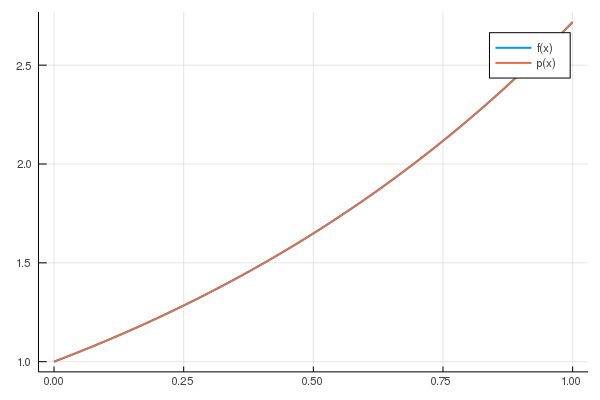
\includegraphics[width=0.5\textwidth]{plots/task5plotf1_5.png}} \hfill
%	\subfloat[2.][$n=10$]{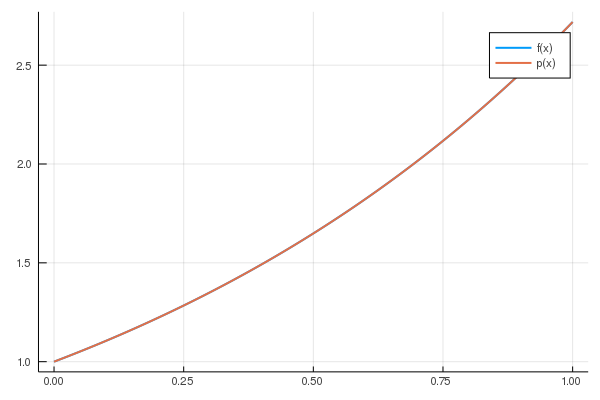
\includegraphics[width=0.5\textwidth]{plots/task5plotf1_10.png}} \hfill
%	\subfloat[3.][$n=15$]{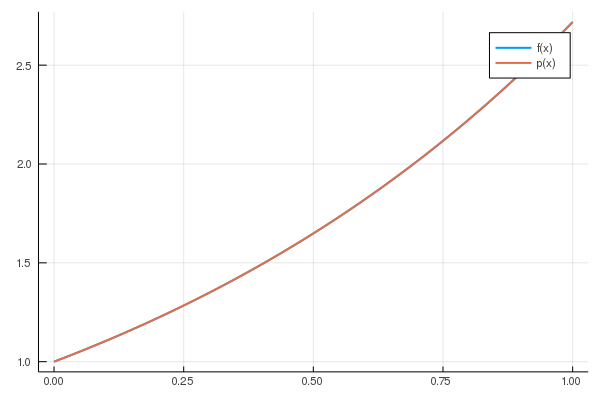
\includegraphics[width=0.5\textwidth]{plots/task5plotf1_15.png}} \hfill
	\caption*{Wykres funkcji $e^{x}$ i jej wielomianu interpolacyjnego dla danego stopnia $n$}
\end{figure}		

\begin{figure}[!htbp]
	\centering
%	\subfloat[1.][$n=5$]{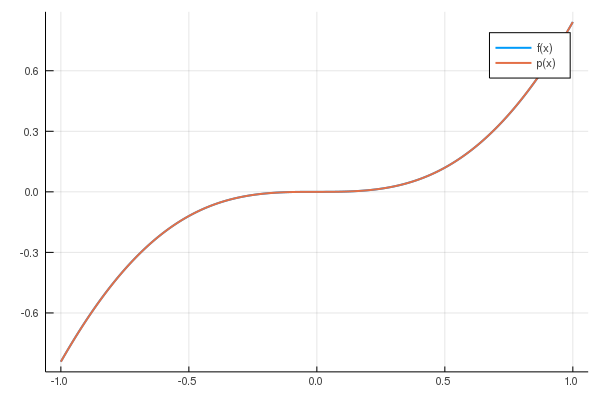
\includegraphics[width=0.5\textwidth]{plots/task5plotf2_5.png}} \hfill
%	\subfloat[2.][$n=10$]{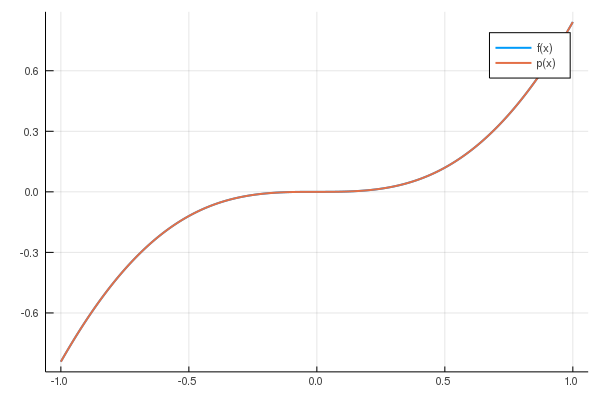
\includegraphics[width=0.5\textwidth]{plots/task5plotf2_10.png}} \hfill
%	\subfloat[3.][$n=15$]{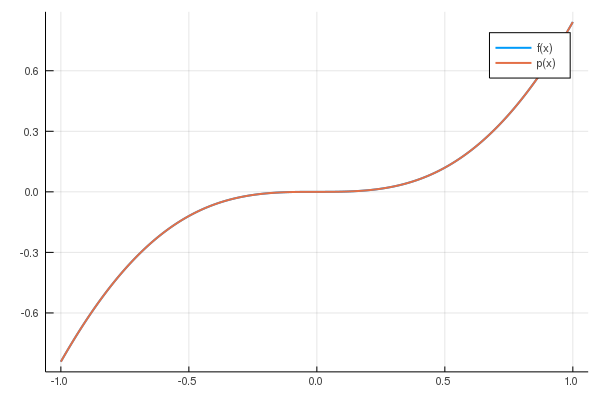
\includegraphics[width=0.5\textwidth]{plots/task5plotf2_15.png}} \hfill
	\caption*{Wykres funkcji $x^2\sin{x}$ i jej wielomianu interpolacyjnego dla danego stopnia $n$}
\end{figure}	





	\clearpage
	
	\section*{Zadanie 6}
	
	Celem zadania było przetestowanie funkcji \texttt{rysujNnfx(f,a,b,n)} (z zadania 4) na następujących przykładach:
	\begin{enumerate}[(a)]
		\item $f(x) = |x|$, $[a, b] = [-1,1]$, $n \in \{5,10,15\}$,
		\item $f(x) = \frac{1}{1+x^2}$, $[a, b] = [-5,5]$, $n \in \{5,10,15\}$.
	\end{enumerate}
Wykresy otrzymane za pomocą metody \texttt{rysujNnfx(f,a,b,n)} prezentują poniższe wykresy.
\begin{figure}[h]
	\centering
%	\subfloat[1.][$n=5$]{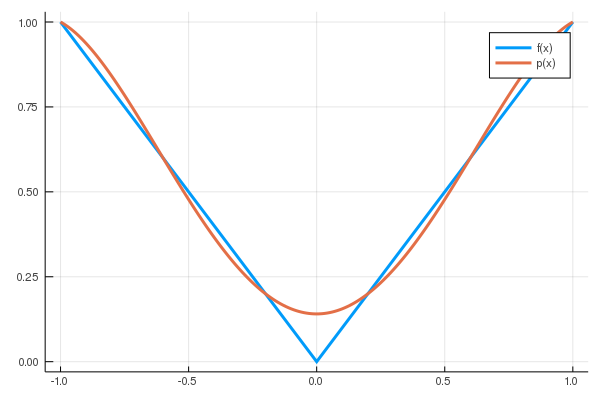
\includegraphics[width=0.5\textwidth]{plots/task6plotf1_5.png}} \hfill
%	\subfloat[2.][$n=10$]{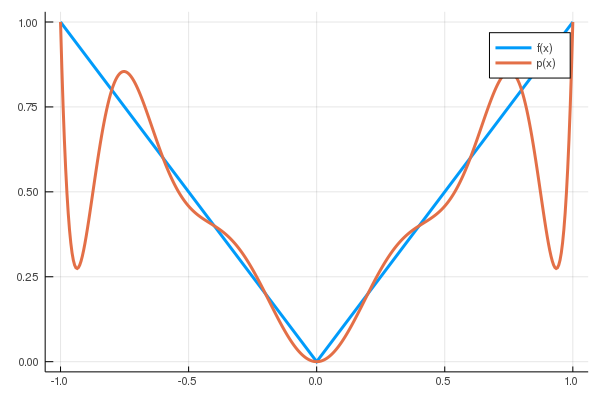
\includegraphics[width=0.5\textwidth]{plots/task6plotf1_10.png}} \hfill
%	\subfloat[3.][$n=15$]{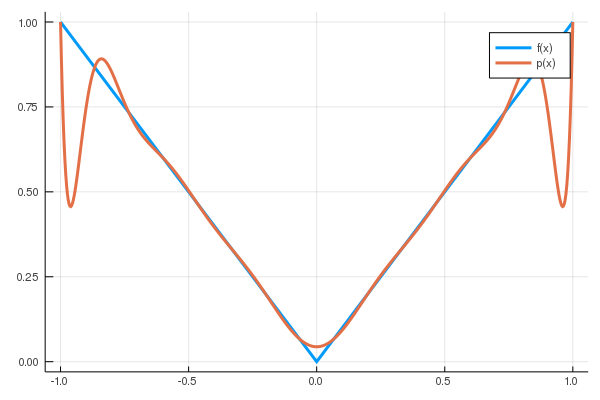
\includegraphics[width=0.5\textwidth]{plots/task6plotf1_15.png}} \hfill
%	\subfloat[4.][$n=20$]{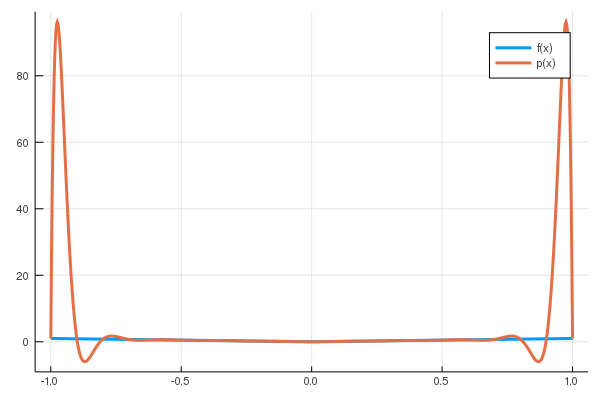
\includegraphics[width=0.5\textwidth]{plots/task6plotf1_20.png}} \hfill
	\caption*{Wykres funkcji $|x|$ i jej wielomianu interpolacyjnego dla danego stopnia $n$}
	\label{fig:3}
\end{figure}		

\begin{figure}[h]
	\centering
%	\subfloat[1.][$n=5$]{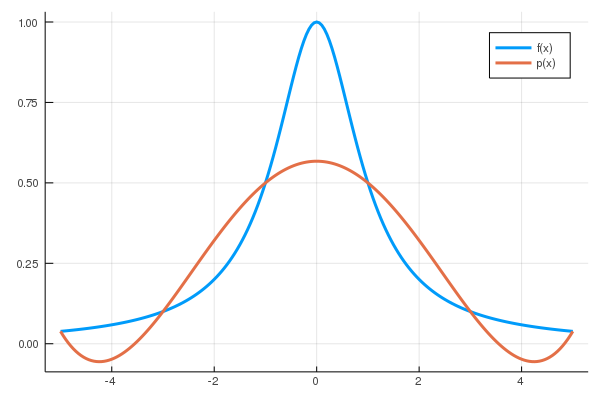
\includegraphics[width=0.5\textwidth]{plots/task6plotf2_5.png}} \hfill
%	\subfloat[2.][$n=10$]{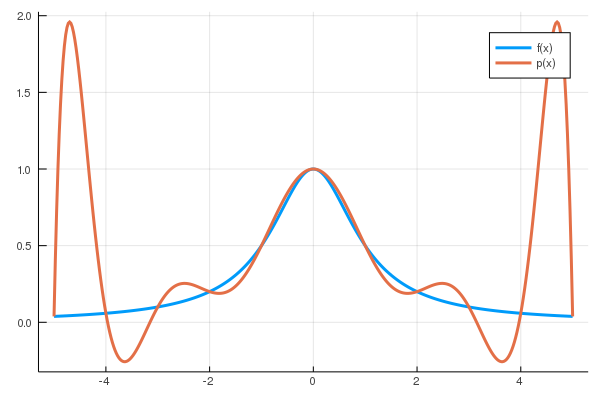
\includegraphics[width=0.5\textwidth]{plots/task6plotf2_10.png}} \hfill
%	\subfloat[3.][$n=15$]{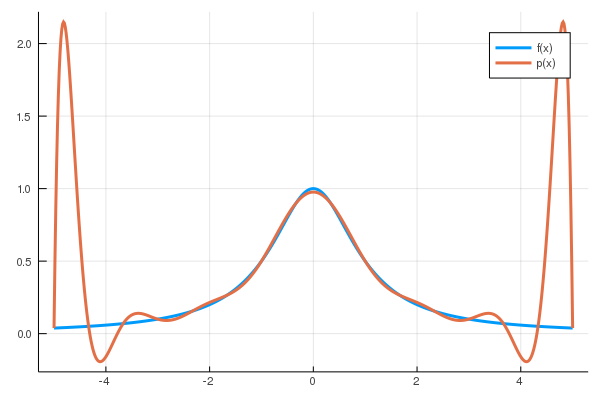
\includegraphics[width=0.5\textwidth]{plots/task6plotf2_15.png}} \hfill
%	\subfloat[4.][$n=20$]{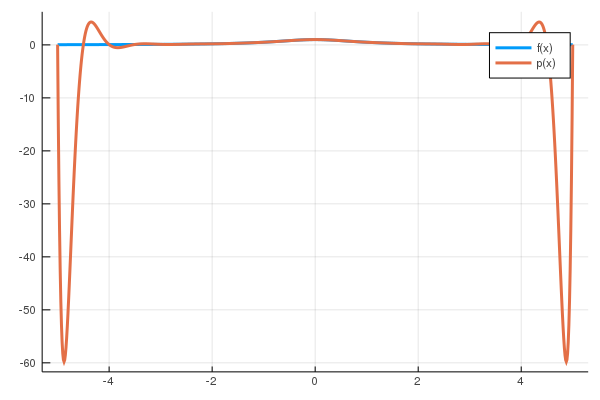
\includegraphics[width=0.5\textwidth]{plots/task6plotf2_20.png}} \hfill
	\caption*{Wykres funkcji $\frac{1}{1+x^2}$ i jej wielomianu interpolacyjnego dla danego stopnia $n$}
	\label{fig:4}
\end{figure}

Widać, że dla funkcji $|x|$ pojawiają się większe odchylenia niż dla funkcji z zadania poprzedniego. Widać też, że wraz ze zwiększaniem stopnia wielomianu odchylenia/błędy, w szczególności na końcach przedziału, znacznie wzrastają. Dla $n=20$ te odchylenia są już na tyle duże, że wykres traci na czytelności. Dla drugiej funkcji sytuacja wygląda tak samo -- wraz ze zwiększaniem stopnia wielomianu błąd rośnie, a błędy najbardziej rosną na końcach przedziału. Jest to sprzeczne z intuicją, ponieważ zwiększajac stopień wielomianu interpolacyjnego oczekujemy lepszego przybliżenia. Zaobserwowane zjawisko nosi nazwę zjawiska Rungego. (Sama funkcja $\frac{1}{1+x^2}$ nazywana jest funkcją Rungego). Polega ono na tym, że dla pewnych funkcji błąd wielomianu
interpolacyjnego wyliczonego za pomocą równoodległych węzłów dąży do nieskończoności wraz ze
wzrostem stopnia tego wielomianu interpolacyjnego.\\
Pojawia się pytanie czy można poprawić dokładność wielomianów interpolacyjnych dla takich funkcji. Z pomocą przychodzą nam węzły Czebyszewa będące pierwiastkami wielomianów Czebyszewa pierwszego rodzaju. Ich użycie zwiększa liczbę węzłów w miejscach, które są trudniejsze do przybliżenia, czyli między innymi na końcach przedziału. Skutkuje to otrzymaniem dokładniejszego przybliżenia. Poniżej znajdują się wykresy z wielomianami interpolacyjnymi stworzonymi na podstawie węzłów Czebyszewa.

\begin{figure}[h]
	\centering
%	\subfloat[1.][$n=5$]{\includegraphics[width=0.5\textwidth]{plots/task6ChebyshevPlotf1_5.png}} \hfill
%	\subfloat[2.][$n=10$]{\includegraphics[width=0.5\textwidth]{plots/task6ChebyshevPlotf1_10.png}} \hfill
%	\subfloat[3.][$n=15$]{\includegraphics[width=0.5\textwidth]{plots/task6ChebyshevPlotf1_15.png}} \hfill
%	\subfloat[4.][$n=20$]{\includegraphics[width=0.5\textwidth]{plots/task6ChebyshevPlotf1_20.png}} \hfill
	\caption*{Wykres funkcji $|x|$ i jej wielomianu interpolacyjnego skonstruowanego przy pomocy węzłów Czebyszewa}
	\label{fig:4}
\end{figure}
\begin{figure}[h]
	\centering
%	\subfloat[1.][$n=5$]{\includegraphics[width=0.5\textwidth]{plots/task6ChebyshevPlotf2_5.png}} \hfill
%	\subfloat[2.][$n=10$]{\includegraphics[width=0.5\textwidth]{plots/task6ChebyshevPlotf2_10.png}} \hfill
%	\subfloat[3.][$n=15$]{\includegraphics[width=0.5\textwidth]{plots/task6ChebyshevPlotf2_15.png}} \hfill
%	\subfloat[4.][$n=20$]{\includegraphics[width=0.5\textwidth]{plots/task6ChebyshevPlotf2_20.png}} \hfill
	\caption*{Wykres funkcji $\frac{1}{1+x^2}$ i jej wielomianu interpolacyjnego stworzonego przy pomocy węzłów Czebyszewa}
	\label{fig:4}
\end{figure}



\end{document}